\documentclass{article}
\usepackage{mathtools}
\usepackage{amssymb}
\usepackage{amsthm}
\usepackage{extarrows}
\usepackage{graphicx}
\usepackage{subcaption}
\usepackage{enumitem}
\title{Assignment 5}
\date{Sepetember 29, 2020}
\author{Haixiang Zhu}
\begin{document}
    \maketitle
    \renewcommand{\arraystretch}{1.2}
    \begin{enumerate}
        \item 
        \begin{enumerate}
            \item Define $V(\cdot)$ to be the value function, $k'$ to be the capital stock chosen today and available for production in next period and $c,k$, respectively, to be the consumption and capital stock available for production in current period.
            $k$ is the state variable and $c,k'$ are the choice variables.\\
            Bellman equation: 
            \begin{align*}
                &V(k)=\max_{c,k'}[u(c)+\beta V(k')]\\
                &\qquad=\max_{c,k'}[\frac{c^{1-\sigma}-1}{1-\sigma}+\beta V(k')]\\
                &\begin{array}{r@{\quad}l}
                    s.t.&c+k'=Ak\\
                    &c\ge0\\
                    &k'\ge0\\
                    &\sigma>0\\
                    &k\enspace\text{given}    
                \end{array}           
            \end{align*}
            \item Inada conditions of the period utility function $(\sigma>0)$:
            \begin{equation*}
                \left\{
                \begin{aligned}
                &\lim_{c\to0}{u}'(c)=\lim_{c\to0}c^{-\sigma}=\infty\\
                &\lim_{c\to\infty}{u}'(c)=\lim_{c\to\infty}c^{-\sigma}=0
                \end{aligned}
            \right.
            \end{equation*}
            Guess:\\
            Consider a one-period problem:\\
            Since $V_0(k)=0$,
            \begin{align*}
                &V_1(k)=\max_{c,k'}[\frac{c^{1-\sigma}-1}{1-\sigma}+\beta\cdot0]\\
                &\begin{array}{r@{\quad}l}
                    s.t.&c+k'=Ak\\
                    &c\ge0\\
                    &k'\ge0\\
                    &\sigma>0\\
                    &k\enspace\text{given}      
                \end{array}           
            \end{align*}
            Because $u(\cdot)$ satisfy the Inada conditions, the consumption constraint will not bind, i.e. $c>0$. By the FOC of $[k']$ and complementary slackness, one can show that the policy functions
            \begin{align*}
                &k'=0\equiv g_1(k)\\
                \Rightarrow&c=Ak\equiv g_1^c(k)\\
                \Rightarrow&V_1(k)=\frac{(Ak)^{1-\sigma}-1}{1-\sigma}
            \end{align*}
            Consider a two-period problem:
                \begin{align*}
                    &V_2(k)=\max_{c,k'}[\frac{c^{1-\sigma}-1}{1-\sigma}+\beta V_1(k')]\\
                    &\qquad\enspace=\max_{c,k'}[\frac{c^{1-\sigma}-1}{1-\sigma}+\beta\frac{(Ak')^{1-\sigma}-1}{1-\sigma}]\\
                    &\begin{array}{r@{\quad}l}
                        s.t.&c+k'=Ak\\
                        &c\ge0\\
                        &k'\ge0\\
                        &\sigma>0\\
                        &k\enspace\text{given}
                    \end{array}
                \end{align*}
            Lagrangian Function:
            \begin{equation*}
                L=\frac{c^{1-\sigma}-1}{1-\sigma}+\beta\frac{(Ak')^{1-\sigma}-1}{1-\sigma}-\lambda(c+k'-Ak)+\nu c+\mu k'
            \end{equation*}
            Necessary Conditions:
            \begin{equation*}
                \left\{\begin{aligned}
                    &\frac{\partial L}{\partial c}=c^{-\sigma}-\lambda+\nu=0\\
                    &\frac{\partial L}{\partial k'}=\beta A^{1-\sigma}(k')^{-\sigma}-\lambda+\mu=0\\
                    &c+k'-Ak=0\\
                    &c\ge0\\
                    &k'\ge0\\
                    &\nu\ge0\\
                    &\mu\ge0\\
                    &\nu c=0\\
                    &\mu k'=0
                \end{aligned}\right.
            \end{equation*}
            Similar to one-period problem, $c>0,\nu=0$. If $k'\to0$, $\beta A^{1-\sigma}(k')^{-\sigma}\to\infty$, which contradicts the FOC of $[k']$. Hence, $k'>0,\mu=0$.\\
            Reduced form:
            \begin{align*}
                &\beta A^{1-\sigma}(k')^{-\sigma}=(Ak-k')^{-\sigma}\\
                \Rightarrow&k'=\frac{(\beta A)^\frac1{\sigma}}{A+(\beta A)^\frac1{\sigma}}Ak\equiv g_2(k)\\
                \Rightarrow&c=Ak-k'=\frac{A}{A+(\beta A)^\frac1{\sigma}}Ak\equiv g_2^c(k)\\
                \Rightarrow&V_2(k)=\frac{(\frac{A}{A+(\beta A)^\frac1{\sigma}}Ak)^{1-\sigma}-1}{1-\sigma}+\beta\frac{(A\frac{(\beta A)^\frac1{\sigma}}{A+(\beta A)^\frac1{\sigma}}Ak)^{1-\sigma}-1}{1-\sigma}
            \end{align*}
            From $V_1(k)$ and $V_2(k)$, we guess the stationary value has the form
            \begin{equation*}
                V(k)=\frac{Xk^{1-\sigma}+Y}{1-\sigma}
            \end{equation*} 
            Verify:\\
            The infinite horizon Bellman equation we are trying to solve is:
            \begin{align*}
                &V(k)=\max_{k'}[\frac{(Ak-k')^{1-\sigma}-1}{1-\sigma}+\beta \frac{X(k')^{1-\sigma}+Y}{1-\sigma}]\\
                &\begin{array}{r@{\quad}l}
                    s.t.&c=Ak-k'\ge0\\
                    &k'\ge0\\
                    &\sigma>0\\
                    &k\enspace\text{given} 
                \end{array}
            \end{align*}
            Lagrangian Function:
            \begin{equation*}
                L=\frac{(Ak-k')^{1-\sigma}-1}{1-\sigma}+\beta \frac{X(k')^{1-\sigma}+Y}{1-\sigma}+\nu(Ak-k')+\mu k'
            \end{equation*}
            Necessary Conditions:
            \begin{equation*}
                \left\{\begin{aligned}
                    &\frac{\partial L}{\partial k'}=-(Ak-k')^{-\sigma}+\beta X(k')^{-\sigma}-\nu+\mu=0\\
                    &Ak-k'\ge0\\
                    &k'\ge0\\
                    &\nu\ge0\\
                    &\mu\ge0\\
                    &\nu(Ak-k')=0\\
                    &\mu k'=0
                \end{aligned}\right.
            \end{equation*}
            Similar to two-period problem, $k'>0,\mu=0$. If $(Ak-k')\to0$, $-(Ak-k')^{-\sigma}\to-\infty$, which contradicts the FOC of $[k']$. Hence, $Ak-k'>0,\nu=0$.\\
            Reduced form:
            \begin{align*}
                &\beta X(k')^{-\sigma}=(Ak-k')^{-\sigma}\\
                \Rightarrow&k'=\frac{(\beta X)^\frac1{\sigma}}{1+(\beta X)^\frac1{\sigma}}Ak\equiv g(k)\\
                \Rightarrow&c=Ak-k'=\frac{1}{1+(\beta X)^\frac1{\sigma}}Ak\equiv g^c(k)\\
                \Rightarrow&V(k)=\frac{\left(\frac{1}{1+(\beta X)^\frac1{\sigma}}Ak\right)^{1-\sigma}-1}{1-\sigma}+\beta\frac{X\left(\frac{(\beta X)^\frac1{\sigma}}{1+(\beta X)^\frac1{\sigma}}Ak\right)^{1-\sigma}+Y}{1-\sigma}\\
                &\qquad=\frac{\left(\frac{A}{1+(\beta X)^\frac1{\sigma}}\right)^{1-\sigma}[1+(\beta X)^\frac1{\sigma}]k^{1-\sigma}+\beta Y-1}{1-\sigma}\\
                &\qquad=\frac{A^{1-\sigma}[1+(\beta X)^\frac1{\sigma}]^\sigma k^{1-\sigma}+\beta Y-1}{1-\sigma}
            \end{align*}
            For the Bellman equation to be satisfied, it must be that this is equal to our guess. We do this by equating coefficients
            \begin{align*}
                &\left\{\begin{aligned}
                    &A^{1-\sigma}[1+(\beta X)^\frac1{\sigma}]^\sigma=X\\
                    &\beta Y-1=Y
                \end{aligned}\right.\\
                \Rightarrow&\left\{\begin{aligned}
                    &X=(A^{\frac{\sigma-1}{\sigma}}-\beta^{\frac{1}{\sigma}})^{-\sigma}\\
                    &Y=\frac{1}{\beta-1}
                \end{aligned}\right.
            \end{align*}
            Hence, the value function is
            \begin{equation*}
                V(k)=\frac{(A^{\frac{\sigma-1}{\sigma}}-\beta^{\frac{1}{\sigma}})^{-\sigma}k^{1-\sigma}}{1-\sigma}+\frac{1}{(1-\sigma)(\beta-1)}
            \end{equation*}
            and the optimal policy function of capital is 
            \begin{align*}
                g(k)&=\frac{(\beta X)^\frac1{\sigma}}{1+(\beta X)^\frac1{\sigma}}Ak\\
                &=\frac{Ak}{1+(\beta X)^{-\frac{1}{\sigma}}}\\
                &=\frac{Ak}{1+[(A^{\frac{\sigma-1}{\sigma}}\beta^{-\frac{1}{\sigma}}-1)^{-\sigma}]^{-\frac{1}{\sigma}}}\\
                &=\frac{Ak}{A^{\frac{\sigma-1}{\sigma}}\beta^{-\frac{1}{\sigma}}}\\
                &=k(A\beta)^{\frac{1}{\sigma}}
            \end{align*}
            The optimal policy function of consumption is
            \begin{equation*}
                g^c(k)=Ak-k'=Ak(1-A^{\frac{1-\sigma}{\sigma}}\beta^{\frac{1}{\sigma}})
            \end{equation*}
            \item 
            \begin{proof}
                \begin{align*}
                    \lim_{\sigma\to1}u(c_t)=&\lim_{\sigma\to1}\frac{c_t^{1-\sigma}-1}{1-\sigma}\\
                    \xlongequal{t=1-\sigma}&\lim_{t\to0}\frac{c^t-1}{t}\\
                    \xlongequal{L'Hopital's\enspace rule}&\lim_{t\to0}c^t\ln(c_t)\\
                    =&\ln(c_t)
                \end{align*}
            \end{proof}
            When $\sigma=1$, the value function is
            \begin{align*}
                \lim_{\sigma\to1}V(k)&=\lim_{\sigma\to1}\frac{(A^{\frac{\sigma-1}{\sigma}}-\beta^{\frac{1}{\sigma}})^{-\sigma}k^{1-\sigma}+(\beta-1)^{-1}}{1-\sigma}\\
                &=(1-\beta)^{-1}\lim_{\sigma\to1}\frac{k^{1-\sigma}-1}{1-\sigma}+\lim_{\sigma\to1}\frac{(A^{\frac{\sigma-1}{\sigma}}-\beta^{\frac{1}{\sigma}})^{-\sigma}+(\beta-1)^{-1}}{(1-\sigma)}\\
                \xlongequal{L'Hopital's\enspace rule}
                \begin{split}
                    &\frac{\ln k}{1-\beta}+\lim_{\sigma\to1}(A^{\frac{\sigma-1}{\sigma}}-\beta^{\frac{1}{\sigma}})^{-\sigma}\\
                    &\cdot\lim_{\sigma\to1}\left[\ln(A^{\frac{\sigma-1}{\sigma}}-\beta^{\frac{1}{\sigma}})+\sigma\frac{A^{\frac{\sigma-1}{\sigma}}\ln(A)\sigma^{-2}+\beta^{\frac{1}{\sigma}}\ln(\beta)\sigma^{-2}}{A^{\frac{\sigma-1}{\sigma}}-\beta^{\frac{1}{\sigma}}}\right]
                \end{split}\\
                &=\frac{\ln k}{1-\beta}+\frac{1}{1-\beta}\left[\ln(1-\beta)+\frac{\ln A+\beta\ln\beta}{1-\beta}\right]\\
            \end{align*}
            and, plugging $\sigma=1$, the optimal policy functions are
            \begin{align*}
                \left\{\begin{aligned}
                &g(k)=\beta Ak\\
                &g^c(k)=(1-\beta)Ak
                \end{aligned}\right.
            \end{align*}
            \item As shown in Figure 1, the dynamic of capital depends on the product of $\beta$ and $A$.
            If $\beta A>1$, $\forall k_0>0$, the capital stock will keep increasing by $\beta A-1$.
            If $\beta A=1$, $\forall k_0>0$, the capital stock will remain unchanged.
            If $\beta A<1$, $\forall k_0>0$, the capital stock will keep decreasing by $1-\beta A$ until $k=0$.
            \begin{figure}[h!]
                \centering
                \begin{subfigure}[b]{.8\linewidth}
                  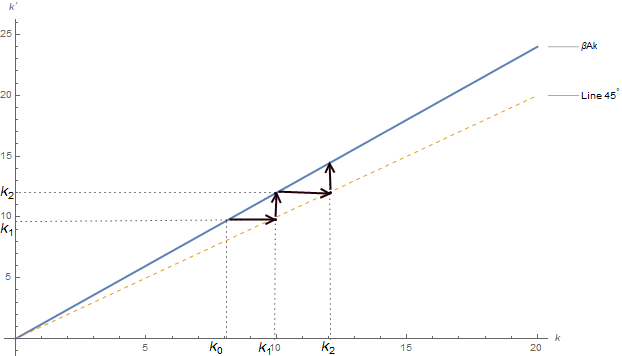
\includegraphics[width=\linewidth]{5_1d1.png}
                   \caption{$\beta A>1$}
                \end{subfigure}
                \begin{subfigure}[b]{.8\linewidth}
                  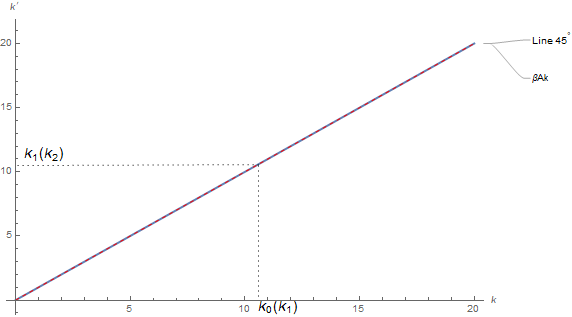
\includegraphics[width=\linewidth]{5_1d2.png}
                  \caption{$\beta A=1$}
                \end{subfigure}
                \begin{subfigure}[b]{.8\linewidth}
                  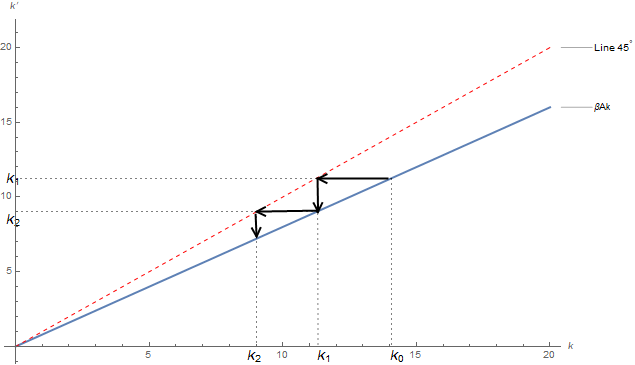
\includegraphics[width=\linewidth]{5_1d3.png}
                  \caption{$\beta A<1$}
                \end{subfigure}
                \caption{The Dynamics of Capital}
            \end{figure}
        \end{enumerate}
        \clearpage
        \item 
        \begin{enumerate}
            \item Budget constraint:
            \begin{equation*}
                b_t+s_t=Rs_{t-1}+w,\quad\forall t=0,1,2,\dots
            \end{equation*}
            where \(s_{-1}=0,b_t,s_t\ge0\)
            \item Dynamic programming problem:\\
            Define $u(\cdot)$ to be the utility function, $V(\cdot)$ to be the value function, $s^-$ to be the bananas saved in last period and $s,b$, respectively, to be the bananas saved and consumed in current period.\\
            $s^-$ is the state variable and $s,b$ are the choice variables.\\
            Bellman equation: 
            \begin{align*}
                &V(s^-)=\max_{b,s}[u(b)+\beta V(s)]\\
                &\begin{array}{r@{\quad}l}
                    s.t.&b+s-Rs^-=w\\
                    &b\ge0\\
                    &s\ge0\\
                    &s^-\enspace\text{given}   
                \end{array}           
            \end{align*}
            \item WLOG, assume that $t=2k,\enspace\forall k=1,2,\dots$
            \begin{align*}
                &\left\{\begin{aligned}
                    &b_t+s_t=Rs_{t-1}+w_H\\
                    &b_{t-1}+s_{t-1}=Rs_{t-2}+w_L
                \end{aligned}\right.\\
                &\Rightarrow b_t+s_t+b_{t-1}+(1-R)s_{t-1}-Rs_{t-2}=w_H+w_L
            \end{align*}
            Dynamic programming problem:\\
            Define $u(\cdot)$ to be the utility function, $V(\cdot)$ to be the value function, $s^=$ to be the bananas saved two period's ago, $s^-,b^-$, respectively, to be the bananas saved and consumed in last period and $s,b$, respectively, to be the bananas saved and consumed in current period.\\
            $b^-,s^-,s^=$ are the state variables and $b,s$ are the choice variables.\\
            Bellman equation: 
            \begin{align*}
                &V(b^-,s^-,s^=)=\max_{b,s}[u(b)+\beta V(b,s,s^-)]\\
                &\begin{array}{r@{\quad}l}
                    s.t.&b+s+b^-+(1-R)s^--Rs^==w_H+w_L\\
                    &b\ge0\\
                    &s\ge0\\
                    &b^-,s^-,s^=\enspace\text{given}  
                \end{array}           
            \end{align*}
        \end{enumerate}
    \end{enumerate}
\end{document}